\section{Más}

\begin{frame}[fragile]{Hoogle}
  Hoogle permite buscar funciones por tipo entre las librerías
  estándar de Haskell:
  
  \begin{center}
  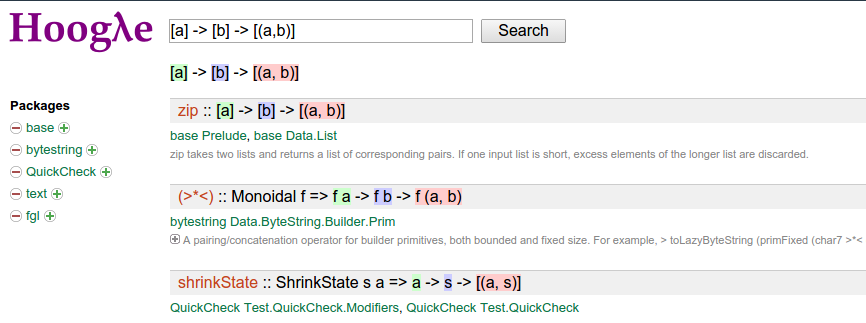
\includegraphics[scale=0.35]{./images/hoogle.png}
  \end{center}
\end{frame}


\begin{frame}[fragile]{Demostraciones}
  Como las funciones no tienen efectos secundarios, podemos razonar la
  corrección del código por inducción:

  \begin{lstlisting}[language=haskell]
qsort []     = []
qsort (x:xs) = qsort [y | y<-xs, y<=x]
            ++ [x]
            ++ qsort [y | y<-xs, y>x]
  \end{lstlisting}

  \textbf{Demostración:} \textit{Quicksort} funciona porque:
  \begin{itemize}
   \item ordena correctamente una lista vacía.
   \item la lista creada mantiene el orden entre las tres partes
  \end{itemize}
\end{frame}


\begin{frame}[fragile]{Idris}
  \textbf{Idris}, construido encima de Haskell, demuestra
  matemáticamente que los
  programas son correctos.
  
  \begin{center}
  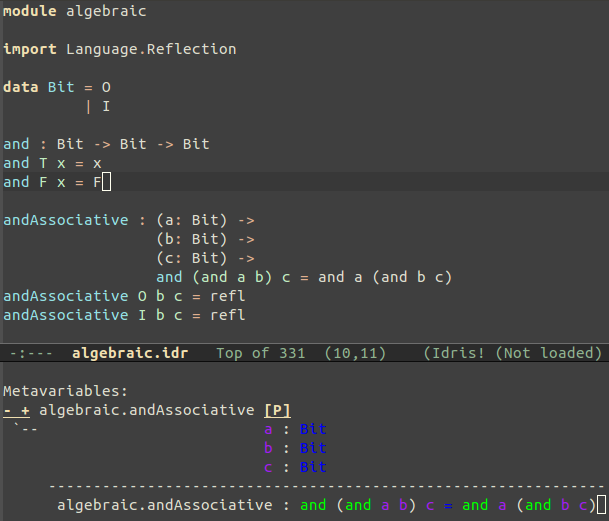
\includegraphics[scale=0.28]{./images/idris.png}
  \end{center}
\end{frame}


\begin{frame}[fragile]{Curry-Howard}
 Los siguientes tipos están habitados:
 \begin{lstlisting}[language=haskell]
 a -> a
 (a,b) -> a
 a -> Either a b
 \end{lstlisting}
 Por las funciones \texttt{id}, \texttt{fst} y \texttt{Left}. 
 Estos, sin embargo, no:
 \begin{lstlisting}[language=haskell]
 a -> b
 a -> (a,b)
 Either a b -> a -> b
 \end{lstlisting}
 
 \textbf{¿Qué tipos de Haskell están habitados?} 
\end{frame}


\begin{frame}[fragile]{Curry-Howard}
 A cada tipo le corresponde una proposición lógica, cambiando:
 \begin{itemize}
  \item \texttt{a -> b} por $a \Rightarrow b$
  \item \texttt{(a,b)} por $a \wedge b$
  \item \texttt{Either a b} por $a \vee b$
  \item \texttt{()} por $True$
  \item \texttt{Void} por $False$
 \end{itemize}

 
 \textbf{¿Qué tipos de Haskell están habitados?} Aquellos cuya
 proposición lógica asociada puede demostrarse verdadera.
\end{frame}